\makeatletter
\def\fps@figure{h}
\makeatother

\hypertarget{intro}{%
\chapter{Intro}\label{intro}}

\begin{itemize}
\item
  Emphasize on the difference between the Solutions Test Framework (E3)
  and the actual Solutions
\item
  The Test Framework is an engineering problem of its own which deals
  with the scaffolding necessary to demonstrate the candidate solutions
  in realistic scenarios
\end{itemize}

\hypertarget{related-work}{%
\chapter{Related work}\label{related-work}}

\begin{itemize}
\item
  There is a huge amount of primitives and partial solutions that are
  relevant to our problem, which makes it difficult to review them all,
  so we will try to design a classification system for them and focus on
  one or two solutions per class while only briefly mentioning their
  alternatives
\item
  Make a distinction between

  \begin{itemize}
  \tightlist
  \item
    primitives - lower level concepts, techniques or frameworks that
    cannot be used as a solution directly, but are used inside higher
    level solutions

    \begin{itemize}
    \tightlist
    \item
      STUN/TURN/ICE
    \item
      Noise Protocol Framework
    \item
      Identity solutions
    \end{itemize}
  \item
    In terms of topology

    \begin{itemize}
    \tightlist
    \item
      Star shaped
    \item
      Peer-to-peer
    \end{itemize}
  \item
    In terms of NAT Traversal

    \begin{itemize}
    \tightlist
    \item
      STUN
    \item
      TURN
    \end{itemize}
  \item
    User/Kernel space
  \item
    In terms of OSI layers:

    \begin{itemize}
    \tightlist
    \item
      Virtual Network Interface Controller - solutions that emulate a
      physical network controller in the OS using TUN/TAP driver. Most
      networked applications are already designed to work with the
      Internet Protocol Stack (Suite - definitions; Stack -
      implementations) in the host operating system and they do not need
      to do anything extra to work with a virtual NIC. Those solutions
      are usually more general purpose as they allow any other
      application on the host machine to use the overlay network.
      Installing an application that also uses this type of a solution
      may be unintuitive because it will essentially install 2 separate
      programs - the actual application and another one that manages the
      virtual network, while the virtual network will not be limited to
      our application but will also be usable by the others.

      \begin{itemize}
      \tightlist
      \item
        IPSec
      \item
        Wireguard
      \item
        Tailscale
      \item
      \end{itemize}
    \item
      Application layer - require the applications to be implemented in
      a way that supports the protocols of the solution by using
      additional libraries or SDKs to facilitate the communications.
      Those solutions result in more purpose built applications as it is
      not possible for an application to use the overlay network if it
      wasn't specifically designed to be able to.

      \begin{itemize}
      \tightlist
      \item
        WebRTC
      \item
        OpenZiti
      \item
      \end{itemize}
    \end{itemize}
  \end{itemize}
\end{itemize}

\hypertarget{osi-model}{%
\chapter{OSI Model}\label{osi-model}}

\begin{itemize}
\tightlist
\item
  Create a figure that maps the various related components to OSI model
  layers
\item
  It can be a ``more or less accurate'' artistic impression since the
  components can cover multiple layers and the layers are somewhat fluid
\end{itemize}

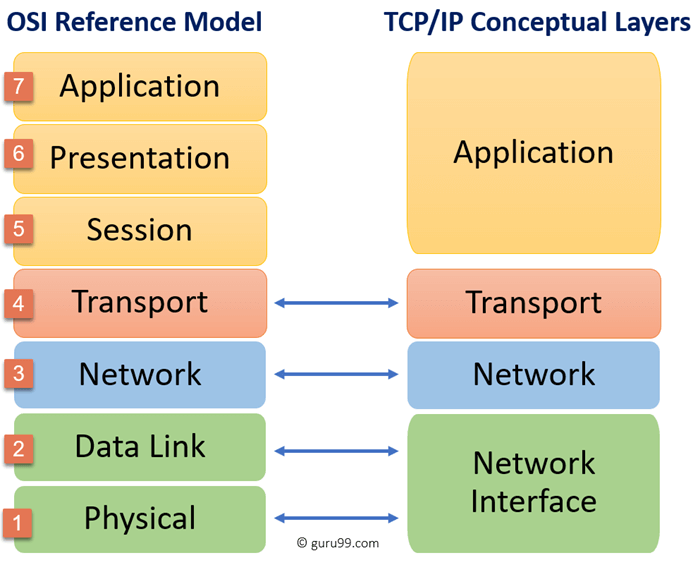
\includegraphics[width=0.5\textwidth,height=0.3\textheight]{notes/../figures/osi-model-2.png}
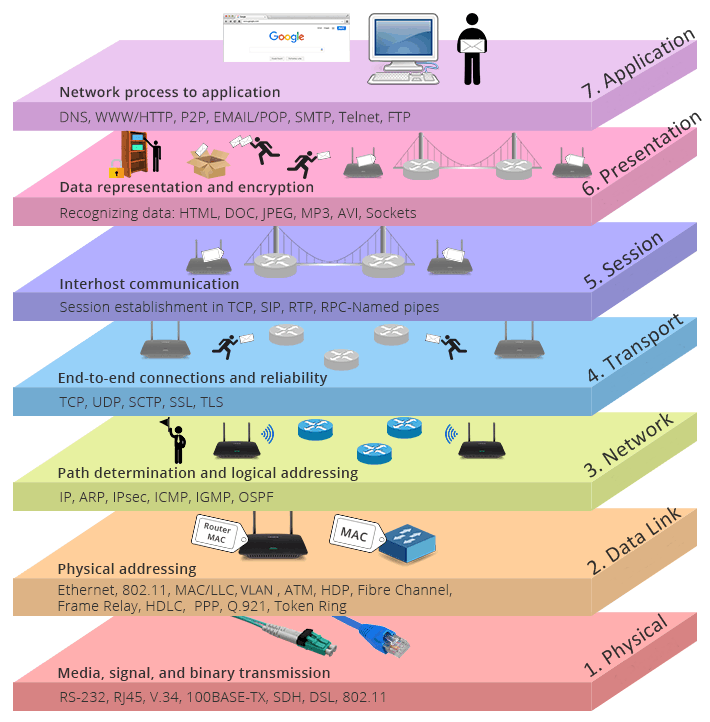
\includegraphics[width=0.4\textwidth,height=0.3\textheight]{notes/../figures/osi-model-1.png}

The Open Systems Interconnection (OSI) model distinguishes 7 layers in
computer networks:

\begin{figure}
\centering
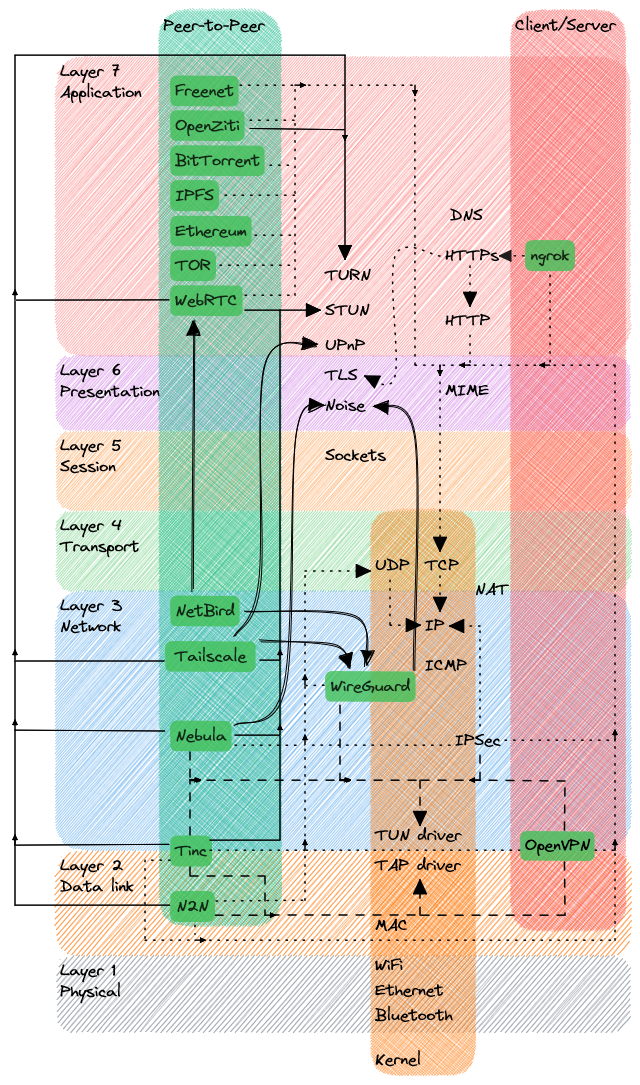
\includegraphics[width=\textwidth,height=0.9\textheight]{notes/../figures/osi-map.excalidraw.png}
\caption{OSI model mapping}
\end{figure}

\newpage

\begin{figure}
\centering
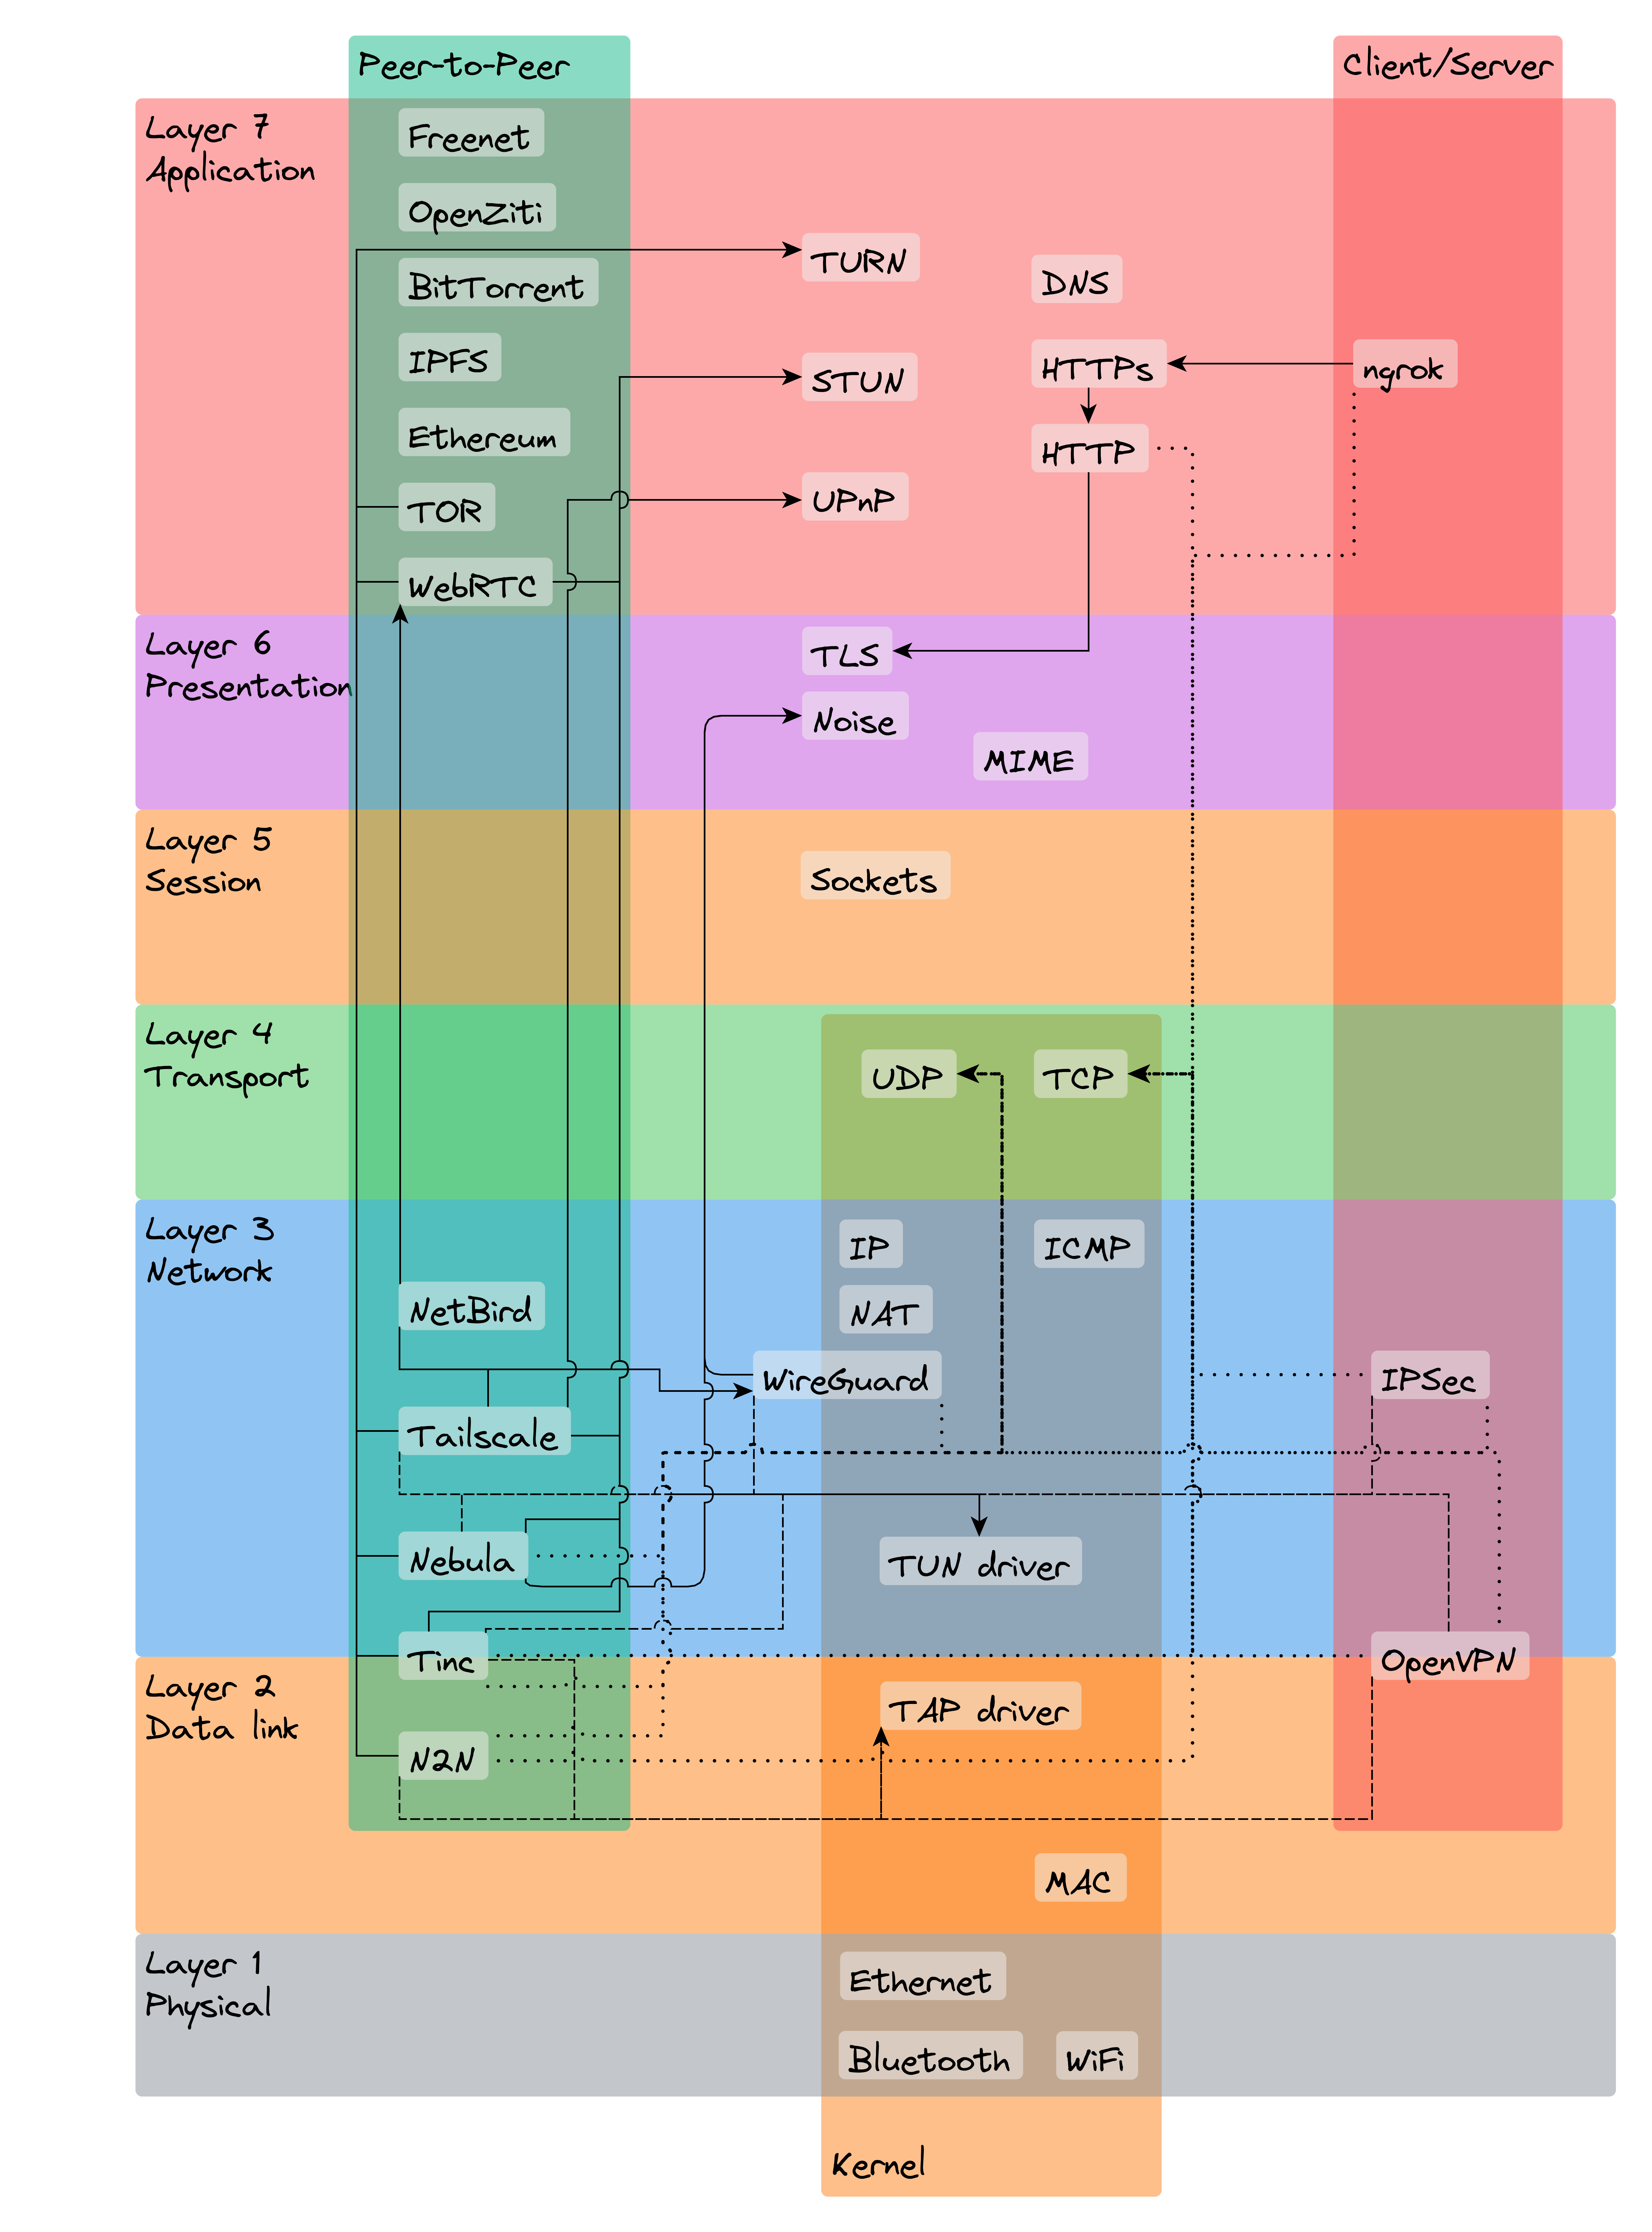
\includegraphics[width=\textwidth,height=0.9\textheight]{notes/../figures/osi-map.yed.png}
\caption{OSI model mapping 2}
\end{figure}

\newpage

\begin{longtable}[]{@{}
  >{\raggedright\arraybackslash}p{(\columnwidth - 6\tabcolsep) * \real{0.0767}}
  >{\raggedright\arraybackslash}p{(\columnwidth - 6\tabcolsep) * \real{0.4390}}
  >{\raggedright\arraybackslash}p{(\columnwidth - 6\tabcolsep) * \real{0.2230}}
  >{\raggedright\arraybackslash}p{(\columnwidth - 6\tabcolsep) * \real{0.2613}}@{}}
\toprule()
\begin{minipage}[b]{\linewidth}\raggedright
OSI Layer
\end{minipage} & \begin{minipage}[b]{\linewidth}\raggedright
Description
\end{minipage} & \begin{minipage}[b]{\linewidth}\raggedright
Protocols
\end{minipage} & \begin{minipage}[b]{\linewidth}\raggedright
Network overlays
\end{minipage} \\
\midrule()
\endhead
7. Application & High level protocols that user-facing services use &
HTTP, HTTPS, DNS, FTP, SMTP, UPnP, NAT-PMP, PCP, SSH, STUN, TURN &
WebRTC, OpenZiti, Teleport, ngrok, TOR, BitTorrent, IPFS, Ethereum,
Freenet \\
\hline 6. Presentation & Translation of data between a networking
service and an application, e.g.~encoding, compression, encryption &
MIME, TLS, Noise & \\
\hline 5. Session & Session setup, management, teardown, authentication,
authorization & SOCKS, X.225 & \\
\hline 4. Transport & Sending data of variable length over a network
while maintaining quality-of-service, e.g.~ports, connections, packet
splitting & UDP, TCP, NAT port mapping & \\
\hline 3. Network & Sending data packets between two nodes, routed via a
path of other nodes, e.g.~addressing, routing & IP, ICMP, NAT & TUN
driver, IPSec, OpenVPN, Tinc, Wireguard, Tailscale, Nebula, ZeroTier \\
\hline 2. Data link & Sending data frames between two nodes, directly
connected via a physical layer, e.g.~on a LAN & MAC, L2TP & TAP driver,
N2N, OpenVPN, Tinc \\
\hline 1. Physical & Sending raw bits over a physical medium & RS232,
Ethernet, WiFi, USB, Bluetooth & \\
\bottomrule()
\end{longtable}

\newpage

\begin{longtable}[]{@{}
  >{\raggedright\arraybackslash}p{(\columnwidth - 10\tabcolsep) * \real{0.1360}}
  >{\raggedright\arraybackslash}p{(\columnwidth - 10\tabcolsep) * \real{0.2000}}
  >{\raggedright\arraybackslash}p{(\columnwidth - 10\tabcolsep) * \real{0.0800}}
  >{\raggedright\arraybackslash}p{(\columnwidth - 10\tabcolsep) * \real{0.0960}}
  >{\raggedright\arraybackslash}p{(\columnwidth - 10\tabcolsep) * \real{0.1280}}
  >{\raggedright\arraybackslash}p{(\columnwidth - 10\tabcolsep) * \real{0.3600}}@{}}
\toprule()
\begin{minipage}[b]{\linewidth}\raggedright
Network overlay
\end{minipage} & \begin{minipage}[b]{\linewidth}\raggedright
Open source
\end{minipage} & \begin{minipage}[b]{\linewidth}\raggedright
OSI Layer
\end{minipage} & \begin{minipage}[b]{\linewidth}\raggedright
Peer-to-Peer
\end{minipage} & \begin{minipage}[b]{\linewidth}\raggedright
NAT Traversal
\end{minipage} & \begin{minipage}[b]{\linewidth}\raggedright
Implementation
\end{minipage} \\
\midrule()
\endhead
IPSec & Yes & Layer 3 & No & & TUN driver \\
\hline OpenVPN & Yes & Layer 2, 3 & No & & TUN or TAP driver \\
\hline Tinc & Yes & Layer 2, 3 & Yes & STUN, TURN & TUN or TAP driver \\
\hline N2N & Yes & Layer 2 & Yes & TURN & TAP driver \\
\hline Wireguard & Yes & Layer 3 & No & & Linux kernel module or TUN
driver; Uses Noise \\
\hline Tailscale & Yes (client); No (server) & Layer 3 & Yes & STUN,
DERP, UPnP & Uses Wireguard \\
\hline Nebula & Yes & Layer 3 & Yes & STUN, TURN & Uses Noise \\
\hline ZeroTier & No & Layer 3 & Yes & STUN, TURN & \\
\hline WebRTC & Yes & Layer 7 & Yes & STUN, TURN & \\
\hline OpenZiti & Yes & Layer 7 & ? & TURN* & \\
\hline Teleport & Yes & Layer 7 & ? & TURN* & \\
\hline ngrok & No & Layer 7 & No & Proxy & \\
\hline TOR & Yes & Layer 7 & Yes & TURN* & \\
\hline BitTorrent & Yes & Layer 7 & Yes & ? & \\
\hline IPFS & Yes & Layer 7 & Yes & ? & \\
\hline Ethereum & Yes & Layer 7 & Yes & ? & \\
\hline Freenet & Yes & Layer 7 & Yes & ? & \\
\bottomrule()
\end{longtable}

\begin{itemize}
\item
  Resources

  \begin{itemize}
  \tightlist
  \item
    \href{https://jvns.ca/blog/2021/05/11/what-s-the-osi-model-/}{The
    OSI model doesn\textquotesingle t map well to TCP/IP}
  \end{itemize}
\end{itemize}

\hypertarget{primitives}{%
\section{Primitives}\label{primitives}}

\hypertarget{internet-protocol}{%
\subsection{Internet Protocol}\label{internet-protocol}}

\begin{itemize}
\item
  IP addresses

  \begin{itemize}
  \tightlist
  \item
    in The Netherlands Ziggo and KPN provide IPv6, but T-Mobile does
    not. Overall \textasciitilde40\% client-side adoption.
  \end{itemize}
\item
  Routing
\item
  DNS
\item
  TLS
\end{itemize}

\hypertarget{network-address-translation-nat-traversal}{%
\subsubsection{Network Address Translation (NAT)
Traversal}\label{network-address-translation-nat-traversal}}

\url{https://bford.info/pub/net/p2pnat/}

\url{https://www.jordanwhited.com/posts/wireguard-endpoint-discovery-nat-traversal/}

\hypertarget{session-traversal-utilities-for-nat-stun}{%
\subsubsection{Session Traversal Utilities for NAT
(STUN)}\label{session-traversal-utilities-for-nat-stun}}

\begin{itemize}
\item
  Uses a STUN server for discovery and UDP hole-punching
\item
  Communications are peer-to-peer
\item
  Examples:

  \begin{itemize}
  \item
    \url{https://github.com/shawwwn/Gole}
  \item
    \url{https://github.com/malcolmseyd/natpunch-go}
  \item
    \url{https://github.com/coturn/coturn} - used in NetBird
  \item
    \url{https://github.com/pion/stun} - used in NetBird
  \item
    \url{https://github.com/ccding/go-stun} - used in Headscale
  \end{itemize}
\end{itemize}

\hypertarget{traversal-using-relays-around-nat-turn}{%
\subsubsection{Traversal Using Relays around NAT
(TURN)}\label{traversal-using-relays-around-nat-turn}}

\begin{itemize}
\item
  Peers use a relay server as a mediator to route traffic
\item
  Examples

  \begin{itemize}
  \item
    \url{https://github.com/coturn/coturn}
  \item
    \url{https://github.com/pion/stun}
  \end{itemize}
\end{itemize}

\hypertarget{universal-plug-and-play-upnp}{%
\subsubsection{Universal Plug and Play
(UPnP)}\label{universal-plug-and-play-upnp}}

\begin{itemize}
\tightlist
\item
  Not always supported
\item
  Often disabled due to security and performance concerns

  \begin{itemize}
  \tightlist
  \item
    Bugs in the UPnP implementation allowing remote attackers from
    outside the local network to configure port forwarding
  \item
    IOT devices

    \begin{itemize}
    \tightlist
    \item
      might expose themselves to the internet via UPnP
    \item
      often designed to prioritize convenience over security
    \item
      sometimes use default admin user/password
    \item
      Too many ports being configured for forwarding might slow down the
      network
    \item
    \end{itemize}
  \end{itemize}
\end{itemize}

\hypertarget{interactive-connectivity-establishment-ice}{%
\subsubsection{Interactive Connectivity Establishment
(ICE)}\label{interactive-connectivity-establishment-ice}}

\begin{itemize}
\tightlist
\item
  Umbrella term covering STUN/TURN and other related techniques
\end{itemize}

\hypertarget{designated-encrypted-relay-for-packets-derp}{%
\subsubsection{Designated Encrypted Relay for Packets
(DERP)}\label{designated-encrypted-relay-for-packets-derp}}

\begin{itemize}
\item
  TURN-like protocol by Tailscale
\item
  Relaying encrypted Wireguard traffic over HTTP
\item
  Routing based on the Peer's public key
\item
  Overview - \url{https://tailscale.com/kb/1232/derp-servers/}
\item
  DERP map - \url{https://login.tailscale.com/derpmap/default}
\item
  Source code

  \begin{itemize}
  \item
    \url{https://github.com/tailscale/tailscale/tree/main/cmd/derper}
  \item
    \url{https://github.com/tailscale/tailscale/blob/main/derp/derp.go}
  \end{itemize}
\end{itemize}

\hypertarget{noise-protocol-framework}{%
\subsection{Noise Protocol Framework}\label{noise-protocol-framework}}

\begin{itemize}
\tightlist
\item
  Framework for building protocols
\item
  Spec - \url{http://www.noiseprotocol.org/noise.pdf}
\item
  Suite of channel establishment protocols
\item
  Similar to TLS
\item
  Based on Elliptic-curve Diffie--Hellman (ECDH) Handshakes
\item
  Used in WhatsApp, Signal, Wireguard
\item
  Resources:

  \begin{itemize}
  \tightlist
  \item
    Crypto Layers

    \begin{itemize}
    \tightlist
    \item
      Low-level primitives - AES, ChaCha20.
    \item
      Usefully combined primitives - AES-OCB, NaCl secretbox\ldots{}
    \item
      High-level protocols - TLS, Noise.
    \item
      (sometimes) crypto spoken over the encrypted protocols, often for
      E2E crypto e.g.~GPG over SMTPS, or CloudFlare blinded CAPTCHA
      tokens over HTTPS
    \end{itemize}
  \item
    \href{https://noiseexplorer.com/}{Design and Explore Noise Handshake
    Patterns}
  \item
    \href{https://duo.com/labs/tech-notes/noise-protocol-framework-intro}{An
    Introduction to the Noise Protocol Framework}
  \item
    \href{https://www.youtube.com/watch?v=ceGTgqypwnQ}{The Noise
    Protocol Framework (Video)}
  \end{itemize}
\end{itemize}

\begin{description}
\item[ChatGPT]
:

TLS (Transport Layer Security) and the Noise Protocol Framework are both
cryptographic protocols that are used to secure communications over the
internet. However, there are some key differences between the two
protocols.

Here are some of the main differences between TLS and the Noise Protocol
Framework:

\begin{enumerate}
\def\labelenumi{\arabic{enumi}.}
\tightlist
\item
  Design Philosophy: TLS is designed to be a general-purpose protocol
  that can be used to secure a wide range of internet communications,
  including web browsing, email, and file transfers. The Noise Protocol
  Framework, on the other hand, is designed to be a lightweight, modular
  protocol that can be easily adapted to different use cases and network
  architectures.
\item
  Cipher Suites: TLS supports a wide range of cipher suites, which are
  combinations of encryption algorithms and key exchange methods. The
  Noise Protocol Framework, on the other hand, supports only a few
  cipher suites that are designed to be secure and efficient.
\item
  Handshake: The TLS handshake is a complex process that involves
  multiple rounds of communication between the client and server. The
  Noise Protocol Framework, on the other hand, has a simpler handshake
  process that involves only a few messages.
\item
  Forward Secrecy: Both TLS and the Noise Protocol Framework support
  forward secrecy, which means that even if an attacker gains access to
  the secret keys used to encrypt communications, they cannot decrypt
  past communications. However, the way that forward secrecy is
  implemented in the two protocols is different.
\item
  Adoption: TLS is widely adopted and supported by most internet
  applications and services. The Noise Protocol Framework is a newer
  protocol that is not yet as widely adopted, although it is gaining
  popularity in certain applications and communities.
\end{enumerate}

Overall, both TLS and the Noise Protocol Framework are effective ways to
secure internet communications. The choice between the two protocols
depends on factors such as the specific use case, the network
architecture, and the desired level of security and efficiency.
\end{description}

\hypertarget{identity}{%
\subsection{Identity}\label{identity}}

\begin{itemize}
\tightlist
\item
  Identity based on a third party Identity Provider (Google, Microsoft,
  Government, \ldots)
\item
  Self Sovereign Identity (SSI)
\end{itemize}

\hypertarget{basic-internet-protocol-solution}{%
\section{Basic Internet Protocol
solution}\label{basic-internet-protocol-solution}}

\begin{itemize}
\tightlist
\item
  Solution with 0 overhead to be used as a reference for the performance
  of the other solutions
\item
  No encryption
\item
  Requires public IP addresses or DNS
\item
  Easy for us to create a demo for measuring the performance because we
  control all of the machines that represent the different parties
\item
  In a real life scenario with separate parties that are not under a
  shared control, it will be difficult to use this solution because it
  requires a lot of manual configuration and coordination between the
  parties
\end{itemize}

\hypertarget{virtual-private-networks-vpns}{%
\subsection{Virtual Private Networks
(VPNs)}\label{virtual-private-networks-vpns}}

\begin{itemize}
\item
  asd
\item
  {[} {]}
\end{itemize}

``A virtual private network {[}4{]} is a secure logical network that is
tunnelled though another network. VPNs are often used for implementing
secure point-to-point communications through the public Internet.
Therefore they usually feature user authentication and content
encryption.'' -- n2n whitepaper

\begin{itemize}
\item
  Traditional centralized VPNs

  \begin{itemize}
  \tightlist
  \item
    OpenVPN
  \item
    IPSec
  \end{itemize}
\item
  Mesh VPNs

  \begin{itemize}
  \tightlist
  \item
    Direct peer-to-peer tunnels between the participants when possible
  \item
    Relaying via an intermediary when necessary
  \item
    Tinc has been around for a long time (first release in 2000)
  \item
    Newer solutions like Tailscale are modernized and more accessible
  \end{itemize}
\item
  Resources:

  \begin{itemize}
  \tightlist
  \item
    \href{https://www.rfc-editor.org/rfc/rfc2764.html}{A Framework for
    IP Based Virtual Private Networks (RFC 2764)}
  \item
  \end{itemize}
\end{itemize}

\hypertarget{wireguard}{%
\section{Wireguard}\label{wireguard}}

\begin{itemize}
\tightlist
\item
  Low level VPN Protocol
\item
  Used by Tailscale
\item
  Whitepaper - \url{https://www.wireguard.com/papers/wireguard.pdf}
\item
  Built with the \href{notes/02022-noise.md}{Noise Protocol Framework}d
\item
  Added to Linux Kernel 5.6 in May 2020
\item
  Typically used as a building block in more complicated systems
\item
  Layer 3 over UDP

  \begin{itemize}
  \tightlist
  \item
    Linux Kernel module

    \begin{itemize}
    \tightlist
    \item
      faster - packets are not copied between kernel memory and
      userspace memory
    \end{itemize}
  \item
    Userspace virtual \href{notes/02021-internet-protocol}{TUN} device

    \begin{itemize}
    \tightlist
    \item
      easier to update because it does not require specific kernel
      modules
    \item
      available on windows
    \end{itemize}
  \end{itemize}
\item
  Simple configuration

  \begin{itemize}
  \tightlist
  \item
    Each peer has a public/private key pair for authentication and
    traffic encryption
  \item
    Each peer has a config file:
  \end{itemize}
\end{itemize}

\newpage

\begin{Shaded}
\begin{Highlighting}[]
\KeywordTok{[Interface]}
\DataTypeTok{Address }\OtherTok{=}\StringTok{ 101.0.0.1/32}
\DataTypeTok{ListenPort }\OtherTok{=}\StringTok{ }\DecValTok{53063}
\DataTypeTok{PrivateKey }\OtherTok{=}\StringTok{ ePTiXXhHjvAHdWUr8Bimk30n0gh3m241RAzsN0JZDW0=}

\KeywordTok{[Peer]}
\DataTypeTok{PublicKey }\OtherTok{=}\StringTok{ BSn0ejd1Y3bKuD+Xpg0ZZeOf+Ies/oql0NZxw+SOmkc=}
\DataTypeTok{AllowedIPs }\OtherTok{=}\StringTok{ 101.0.0.2/32}
\DataTypeTok{Endpoint }\OtherTok{=}\StringTok{ 142.93.135.154:38133}
\DataTypeTok{PersistentKeepalive }\OtherTok{=}\StringTok{ }\DecValTok{25}
\end{Highlighting}
\end{Shaded}

\begin{itemize}
\tightlist
\item
  Creates a virtual network interface in the operating system that looks
  like an additional network card and can be used for TCP/IP
  communications
\item
  Handles the encryption of traffic

  \begin{itemize}
  \tightlist
  \item
    deals with handshakes and generating symmetric session keys
  \end{itemize}
\item
  Cryptokey routing - associates public/private key pairs with IP
  addresses
\item
  Out of scope:

  \begin{itemize}
  \tightlist
  \item
    key distribution - managed manually or via other software that
    builds on top of wireguard
  \item
    peer discovery - for each pair of peers, one needs to have an
    endpoint that can be reached by the other peer
  \end{itemize}
\item
  Resources

  \begin{itemize}
  \tightlist
  \item
    \href{https://blogs.keysight.com/blogs/tech/nwvs.entry.html/2022/09/22/wireguard_the_next-genvpnprotocol-OcEz.html}{WireGuard:
    The Next-Gen VPN Protocol}
  \item
    \href{https://www.jordanwhited.com/posts/wireguard-endpoint-discovery-nat-traversal/}{WireGuard
    Endpoint Discovery and NAT Traversal using DNS-SD}
  \item
    \href{https://git.kernel.org/pub/scm/linux/kernel/git/torvalds/linux.git/commit/?id=e7096c131e5161fa3b8e52a650d7719d2857adfd}{Kernel
    Commit}
  \item
    \href{https://wiki.archlinux.org/title/WireGuard}{Arch Linux Wiki}
  \item
    Examples:
  \item
    https://github.com/takutakahashi/wg-connect
  \item
    https://github.com/stv0g/cunicu
  \item
  \end{itemize}
\end{itemize}

\hypertarget{tailscale}{%
\section{Tailscale}\label{tailscale}}

\begin{itemize}
\tightlist
\item
  Mesh VPN
\item
  Built on top of \href{notes/02051-wireguard.md}{Wireguard}
\item
  Coordination service

  \begin{itemize}
  \tightlist
  \item
    Closed source
  \item
    Facilitates
    \href{notes/0202-nat\#Session\%20Traversal\%20Utilities\%20for\%20NAT\%20(STUN)}{STUN}/\href{notes/02021-internet-protocol.md\#test}{TURN}
    for peer discovery and NAT traversal
  \item
    Distributes wireguard public keys
  \item
    Magic DNS
  \end{itemize}
\item
  Client

  \begin{itemize}
  \tightlist
  \item
    Open source
  \item
    Interacts with the Coordination service
  \item
    Configures Wireguard
  \end{itemize}
\item
  Implementations based on Tailscale

  \begin{itemize}
  \tightlist
  \item
    Tailnet per party

    \begin{itemize}
    \tightlist
    \item
      Parties have their own tailscale accounts and manage their own
      tailnet
    \item
      Each party shares adds the machine they will use for MPC to their
      tailnet
    \item
      They share that machine with the tailnets of the other parties
    \end{itemize}
  \item
    ``Host'' party manages a tailnet

    \begin{itemize}
    \tightlist
    \item
      The host party creates authorization keys for the machines of the
      other parties
    \item
      Each party runs the tailscale client with their authorization key
      which lets them join the host party's tailnet
    \end{itemize}
  \end{itemize}
\end{itemize}

\hypertarget{headscale}{%
\section{Headscale}\label{headscale}}

\begin{itemize}
\tightlist
\item
  Mostly the same as Tailscale, but with an open source coordination
  service that must be self-hosted
\item
  Describe the differences in the deployment and how it affects
  usability
\item
  We implemented a headscale based solution in order to be able to gain
  some insights into how they deal with peer discovery via STUN/TURN and
  configure Wireguard, and whether we can modify it or use parts of it
  in our own custom solution that is a better fit for ad hoc mpc
  sessions.
\end{itemize}

\hypertarget{nebula}{%
\section{Nebula}\label{nebula}}

\begin{itemize}
\tightlist
\item
  \href{https://github.com/slackhq/nebula}{Open source} Mesh VPN
\item
  Similar to Tailscale
\item
  Does not use Wireguard
\item
  NAT traversal via Lighthouses
\item
  Built using the \href{notes/02022-noise}{Noise Protocol Framework}
  (used in Wireguard)
\item
  Uses a Certificate Authority that needs to sign each Peer's
  certificate

  \begin{itemize}
  \tightlist
  \item
    Certificates contain

    \begin{itemize}
    \tightlist
    \item
      Peer's Virtual IP address
    \item
      Peer's public key
    \end{itemize}
  \end{itemize}
\end{itemize}

\hypertarget{zerotier}{%
\section{ZeroTier}\label{zerotier}}

\begin{itemize}
\tightlist
\item
  Closed source Mesh VPN
\item
  Similar to Tailscale
\item
  Does not use Wireguard
\item
\end{itemize}

\hypertarget{n2n}{%
\section{N2N}\label{n2n}}

\begin{itemize}
\tightlist
\item
  \href{https://github.com/ntop/n2n}{Open source} Mesh VPN
\item
  Initial release - 27.03.2008
\item
  Layer 2 \href{notes/02021-internet-protocol}{TAP} in userspace over
  Layer 3

  \begin{itemize}
  \tightlist
  \item
    offers a virtual ethernet jack
  \item
    virtual devices have MAC addresses
  \item
    Multicast/broadcast via the Supernode
  \end{itemize}
\item
  Similar to Nebula
\item
  Does not use Wireguard
\item
  Does not use the Noise protocol
\item
  NAT traversal by relaying via Supernodes

  \begin{itemize}
  \tightlist
  \item
    No STUN - https://github.com/ntop/n2n/issues/57
  \end{itemize}
\item
  Resources:

  \begin{itemize}
  \tightlist
  \item
    \href{http://luca.ntop.org/n2n.pdf}{Whitepaper}
  \end{itemize}
\end{itemize}

\hypertarget{tinc}{%
\section{Tinc}\label{tinc}}

\begin{itemize}
\tightlist
\item
  Mesh VPN released in 2000
\item
  Less modern
\item
  Fewer features
\item
  Slower development
\item
  More academic
\item
  Runs in userspace as a TAP device
\item
  Resources:

  \begin{itemize}
  \tightlist
  \item
    \href{https://www.tinc-vpn.org/documentation-1.1/tinc.pdf}{Manual}
  \end{itemize}
\end{itemize}

\hypertarget{netbird}{%
\section{Netbird}\label{netbird}}

\begin{itemize}
\tightlist
\item
  WireGuard VPN
\item
  NAT Traversal

  \begin{itemize}
  \tightlist
  \item
    Client library - https://github.com/pion/ice
  \item
    STUN/TURN server - https://github.com/coturn/coturn
  \end{itemize}
\item
  Resources:

  \begin{itemize}
  \tightlist
  \item
    Source code - https://github.com/netbirdio/netbird
  \end{itemize}
\end{itemize}

\hypertarget{didcomm-v2}{%
\section{DIDComm v2}\label{didcomm-v2}}

\begin{itemize}
\tightlist
\item
  Protocol for communicating that uses DID for identity management
\item
  Spec: \url{https://identity.foundation/didcomm-messaging/spec/}
\item
  No sessions

  \begin{itemize}
  \tightlist
  \item
    messages are always encrypted with the public keys of the peers
  \end{itemize}
\item
  Routing happens via mediators
\item
  Resources:

  \begin{itemize}
  \tightlist
  \item
    \href{https://newsletter.impervious.ai/decentralized-identifiers-implications-for-your-data-payments-and-communications-2/}{Decentralized
    Identifiers: Implications for Your Data, Payments and
    Communications}
  \end{itemize}
\end{itemize}

\hypertarget{ngrok}{%
\section{ngrok}\label{ngrok}}

\begin{itemize}
\tightlist
\item
  Paid service for creating public URLs for local services
\item
  Never peer-to-peer
\item
  The traffic always goes through their centralized service
\item
\end{itemize}

\hypertarget{ethereums-p2p-protocol}{%
\section{Ethereum's P2P Protocol}\label{ethereums-p2p-protocol}}

\hypertarget{ipfs}{%
\section{IPFS}\label{ipfs}}

\begin{itemize}
\tightlist
\item
  Content Addressable Storage
\item
  Network is for discovering data, not for executing computations
\item
\end{itemize}

\hypertarget{tor}{%
\section{TOR}\label{tor}}

\begin{itemize}
\tightlist
\item
  The Onion Router has the concept of Onion Services, which receive an
  address under the .onion pseudo top level domain and correspond to a
  public key
  (e.g.~vww6ybal4bd7szmgncyruucpgfkqahzddi37ktceo3ah7ngmcopnpyyd.onion)
\item
  Can be used as a privacy layer in other solutions to hide the real IP
  addresses of the parties
\end{itemize}

\hypertarget{freenet}{%
\section{Freenet}\label{freenet}}

\begin{itemize}
\tightlist
\item
  \href{https://homepage.divms.uiowa.edu/~ghosh/freenet.pdf}{Whitepaper}
\item
  Friend2Friend network
\item
  Peer to Peer Dark Web network
\item
  Network that directly connects the machines of people who know each
  other
\item
  Services and files accessible only by other people on the network
\item
  Application layer
\item
  Similar software:

  \begin{itemize}
  \tightlist
  \item
    retroshare
  \item
    gnunet
  \item
    waste
  \item
    peerkeep
  \item
    camlistore
  \end{itemize}
\end{itemize}

\hypertarget{teleport}{%
\section{Teleport}\label{teleport}}

\begin{itemize}
\tightlist
\item
  Layer 7
\item
\end{itemize}

\hypertarget{bittorrent}{%
\section{BitTorrent}\label{bittorrent}}

\begin{itemize}
\tightlist
\item
  No concept of identity based communication or peer discovery
\end{itemize}

\hypertarget{webrtc}{%
\section{WebRTC}\label{webrtc}}

\begin{itemize}
\tightlist
\item
  Peer to peer communications for browsers

  \begin{itemize}
  \tightlist
  \item
    can also work without a browser
  \item
    Mainly used for multimedia communications - Peer-to-peer
    Audio/Video/VoIP
  \end{itemize}
\item
  Spec -
  \href{https://www.w3.org/TR/webrtc/\#persistent-information-exposed-by-webrtc}{https://www.w3.org/TR/webrtc/}
\item
  Uses \href{notes/02021-internet-protocol.md}{nat} STUN/TURN/ICE
\item
  Data is encrypted
\item
  Privacy and Security Considerations

  \begin{itemize}
  \tightlist
  \item
    https://www.w3.org/TR/webrtc/\#privacy-and-security-considerations
  \item
    Revealing IP addresses

    \begin{itemize}
    \tightlist
    \item
      https://www.w3.org/TR/webrtc/\#revealing-ip-addresses
    \item
      For direct communication, the peer's IP addresses are shared
    \item
      Possible to only use TURN servers
    \end{itemize}
  \end{itemize}
\item
  Identity

  \begin{itemize}
  \tightlist
  \item
    Session Description Protocol (SDP)
  \item
    peer certificates are generated and announced over SDP
  \item
    ICE Candidates are negotiated for STUN/TURN connections
  \end{itemize}
\item
  Not a VPN

  \begin{itemize}
  \tightlist
  \item
    I think it can't serve as a TCP/IP network overlay that other
    applications can use
  \end{itemize}
\item
  Does not require additional plugins or native apps
\item
  Perhaps it can be used with PyScript or WebAssembly to run MPyC
  programs in the browser?
\item
  We could design a solution based on WebRTC in a browser by compiling
  the MPyC demos to web assembly or using PyScript.

  \begin{itemize}
  \tightlist
  \item
    https://www.win.tue.nl/\textasciitilde berry/mpyc/pyscript.html
  \item
    https://pyscript.net/
  \end{itemize}
\item
  There seem to be many publicly available services that can be used as
  ICE servers for WebRTC

  \begin{itemize}
  \tightlist
  \item
    \href{http://stun.l.google.com:19302/}{stun.l.google.com:19302}
  \item
    \url{https://gist.github.com/zziuni/3741933}
  \end{itemize}
\item
  Examples

  \begin{itemize}
  \tightlist
  \item
    \url{https://github.com/pion/webrtc}
  \item
    https://github.com/pion/awesome-pion
  \item
    \url{https://github.com/pojntfx/weron}
  \item
    https://github.com/takutakahashi/wg-connect
  \item
    https://github.com/stv0g/cunicu
  \item
    https://github.com/gavv/webrtc-cli
  \item
    https://github.com/szpnygo/gtc
  \item
    https://github.com/cretz/webrtc-ipfs-signaling
  \item
    https://github.com/pion/example-webrtc-applications
  \item
    https://github.com/pion/webrtc/tree/master/examples
  \end{itemize}
\item
  Resources

  \begin{itemize}
  \tightlist
  \item
    \url{https://webrtcforthecurious.com/}
  \item
    \url{https://temasys.io/guides/developers/webrtc-ice-sorcery/}
  \item
    \href{https://web.dev/webrtc-basics/\#toc-rtcpeerconnection}{https://web.dev/webrtc-basics/}
  \end{itemize}
\end{itemize}

\hypertarget{openziti}{%
\section{OpenZiti}\label{openziti}}

\begin{itemize}
\tightlist
\item
  Network Overlay
\item
  No STUN
\item
  Works by relaying traffic through intermediaries
\item
  Focused on Services
\item
  Allows embedding into apps via an SDK
\item
  Tunneler is a proxy that allows non-ziti aware applications to use the
  overlay network by intercepting their traffic
\end{itemize}

\hypertarget{implementation-notes}{%
\chapter{Implementation notes}\label{implementation-notes}}

\hypertarget{headscale}{%
\section{Headscale}\label{headscale}}

\begin{itemize}
\tightlist
\item
  Docker seems to have a 50-100\% performance penalty (possibly due to
  docker's internal NAT) which makes the performance results of the
  headscale setup worse than they should be
\item
  Modify the deployment setup to

  \begin{itemize}
  \tightlist
  \item
    not depend on all machines being on the same tailscale network
  \item
    use the \texttt{*.demo.mpyc.tech} hostnames
  \item
    the nodes should switch between the tailscale and headscale network
    depending on the demo script
  \item
  \end{itemize}
\end{itemize}

\hypertarget{web-browser-python}{%
\section{Web Browser Python}\label{web-browser-python}}

\hypertarget{overview}{%
\subsection{Overview}\label{overview}}

\begin{itemize}
\tightlist
\item
  https://github.com/flexxui/flexx/wiki/PyScript-vs-X
\item
  https://pythondev.readthedocs.io/wasm.html
\item
  https://stromberg.dnsalias.org/\textasciitilde strombrg/pybrowser/python-browser.html
\item
  https://realpython.com/brython-python-in-browser/\#exploring-alternatives-to-brython
\end{itemize}

\hypertarget{transpilers}{%
\subsection{Transpilers}\label{transpilers}}

\begin{figure}
\centering
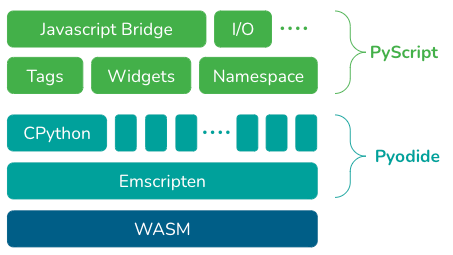
\includegraphics{notes/../figures/pyodide-pyscript.png}
\caption{Alt text}
\end{figure}

Compile Python to JS or WebAssembly (WASM)

\begin{itemize}
\item
  WASM

  \begin{itemize}
  \tightlist
  \item
    www.webassembly.guide/
  \end{itemize}
\item
  PyScript

  \begin{itemize}
  \tightlist
  \item
    https://pyscript.net
  \item
    https://github.com/pyscript/pyscript
  \item
    https://docs.pyscript.net/latest/reference/faq.html
  \item
    https://docs.pyscript.net/latest/guides/asyncio.html
  \item
    PyScript is built using Pyodide, the WebAssembly port of CPython,
    which is compiled using Emscripten.
  \item
    Depends on a python runtime

    \begin{itemize}
    \tightlist
    \item
      Pyodide (Default)

      \begin{itemize}
      \tightlist
      \item
        needs to load a 10 mb runtime
      \end{itemize}
    \item
      MicroPython

      \begin{itemize}
      \tightlist
      \item
        https://pyscript.net/tech-preview/micropython/about.html
      \item
        https://github.com/micropython/micropython
      \item
        More limited, but faster startup
      \end{itemize}
    \end{itemize}
  \item
    Adds

    \begin{itemize}
    \item
      config.toml - configure extra packages to be loaded with pyodide
    \item
    \item
      XWorker
    \item
      other HTML plugins
    \end{itemize}
  \end{itemize}
\item
  Pyodide

  \begin{itemize}
  \tightlist
  \item
    https://github.com/pyodide/pyodide
  \item
    CPython distribution for WASM
  \end{itemize}
\item
  https://github.com/bytecodealliance/wasmtime-py
\item
  Python 3.11.0 for WASM https://github.com/dbaeumer/python-3.11.0
\item
  Transcrypt

  \begin{itemize}
  \tightlist
  \item
    https://www.transcrypt.org
  \item
    https://github.com/TranscryptOrg/Transcrypt
  \item
    https://github.com/bunkahle/Transcrypt-Examples/tree/master/hello
  \item
    Transpile Python to JS ahead of time, include the JS version in the
    Web Page
  \end{itemize}
\item
  PyJS - http://pyjs.org
\item
  Batavia - Unmaintained, moved to PyScript

  \begin{itemize}
  \tightlist
  \item
    https://github.com/beeware/batavia
  \item
    https://batavia.readthedocs.io/en/latest/background/faq.html
  \item
    VM in JS for running CPython bytecode
  \end{itemize}
\item
  RapydScript

  \begin{itemize}
  \tightlist
  \item
    https://github.com/atsepkov/RapydScript
  \end{itemize}
\end{itemize}

\hypertarget{interpreters}{%
\subsection{Interpreters}\label{interpreters}}

Interpreters for python in JS

\begin{itemize}
\tightlist
\item
  Brython

  \begin{itemize}
  \tightlist
  \item
    https://www.brython.info/speed\_results.html
  \item
    Python 3
  \item
    https://brython.info/static\_doc/en/intro.html
  \item
    https://brython.info/static\_doc/en/faq.html
  \end{itemize}
\item
  Skulpt

  \begin{itemize}
  \tightlist
  \item
    https://github.com/skulpt/skulpt/tree/master
  \item
    https://skulpt.org
  \item
    https://skulpt.org/docs/index.html
  \item
    Python 2
  \end{itemize}
\item
  Emscripten??

  \begin{itemize}
  \tightlist
  \item
    https://emscripten.org/docs/introducing\_emscripten/about\_emscripten.html
  \item
    Emscripten is a complete compiler toolchain to WebAssembly, using
    LLVM
  \end{itemize}
\end{itemize}

\hypertarget{brainstorm-for-custom-solutions}{%
\chapter{Brainstorm for custom
solutions}\label{brainstorm-for-custom-solutions}}

\begin{itemize}
\tightlist
\item
  Initial state

  \begin{itemize}
  \tightlist
  \item
    Here's my identity, here are the identities of the other parties
  \end{itemize}
\item
  Desired result

  \begin{itemize}
  \tightlist
  \item
    Executed MPC
  \end{itemize}
\end{itemize}

With tailscale we'd need to

\begin{itemize}
\tightlist
\item
  Each party:

  \begin{itemize}
  \tightlist
  \item
    registers a Tailscale account
  \item
    Downloads and installs tailscale on the machine they want to run the
    MPC on
  \item
    Runs tailscale on their machine and logs into their account in order
    to link it to their own Tailnet
  \item
    Shares their Tailscale machine with the Tailnets of each of the
    other parties
  \item
    Downloads the demo they want to run
  \item
    Form the flags for running the chosen demo

    \begin{itemize}
    \tightlist
    \item
      add -P \$HOST:\$PORT for each party using their Tailscale
      hostname/virtual IP
    \end{itemize}
  \item
    Run the demo
  \end{itemize}
\end{itemize}

\begin{center}\rule{0.5\linewidth}{0.5pt}\end{center}

\begin{itemize}
\tightlist
\item
  we don't need to use the same route for the communication Party A →
  Party B and Party B → Party A
\item
  we can have something like an asynchronous STUN
\item
  Party A sends a QR code/public URL/json object/DID document containing

  \begin{itemize}
  \tightlist
  \item
    Party A's public key
  \item
    Party A's Mediator URL
  \end{itemize}
\item
  The mediator is a STUN/TURN/DERP server

  \begin{itemize}
  \tightlist
  \item
    other parties can either use it as a STUN server to find out how to
    access the hole in party A's NAT punched by the mediator
  \item
    or use it as a relayer so that Party B can send encrypted packets to
    party A via the mediator
  \end{itemize}
\item
  Instead of a QR code, the information could be stored on a public
  ledger and could be resolved via DIDs
\end{itemize}

\begin{center}\rule{0.5\linewidth}{0.5pt}\end{center}

\begin{itemize}
\tightlist
\item
  There is a generic MPC wrapper program that deals with supporting
  tasks like generating identities and pulling MPC demos
\item
  One party creates a ``lobby'' for an MPC session in their program and
  get a session id/public URL/QR code that can be shared with the other
  parties
\item
\end{itemize}

\begin{center}\rule{0.5\linewidth}{0.5pt}\end{center}

\begin{itemize}
\tightlist
\item
  Public Website is visited by everyone
\item
  They prove their identities using a SSI wallet or OIDC
\item
  They get a QR code that serves as an invitation

  \begin{itemize}
  \tightlist
  \item
    contains their STUN based endpoint and identity
  \end{itemize}
\item
  Somehow everyone needs to scan each other's qr codes
\end{itemize}

\begin{center}\rule{0.5\linewidth}{0.5pt}\end{center}

\begin{center}\rule{0.5\linewidth}{0.5pt}\end{center}

\begin{center}\rule{0.5\linewidth}{0.5pt}\end{center}

\begin{itemize}
\tightlist
\item
  One party creates a ``lobby'' for an MPC session by visiting a public
  website

  \begin{itemize}
  \tightlist
  \item
    They provide their identity via OIDC/SSI wallet
  \end{itemize}
\item
  They get a public link/QR code that can be shared with the other
  parties
\item
  The parties visit the URL and also provide their identities
\item
  The parties obtain the MPC program they want to run

  \begin{itemize}
  \tightlist
  \item
    MPC program distribution could be done separately via cloning the
    github repo?
  \item
    They could choose a DEMO and download it from the website?
  \item
    There could also be a program running on the host machines that
    deals with the source code distribution. Similar to downloading
    custom maps for warcraft 3 or dota 2?
  \item
    They could specify the source code when creating the MPC session in
    the website?
  \item
    If the demo is not symmetrical where different parties have
    different roles and need to execute different programs, the roles
    could be assigned by the host or the people could choose their
    preferred role themselves?
  \end{itemize}
\item
  The parties download a configuration file that contains information on
  how to connect to the other parties
\item
  They run the demos with the downloaded config file
\item
  A temporary Wireguard mesh VPN is created between all parties
\end{itemize}

\hypertarget{writing}{%
\chapter{Writing}\label{writing}}

\begin{itemize}
\item
  Ask questions and answer them
\item
  Don't try to get the writing perfect on the first pass
\item
  Write anything first and then iterate on it later
\item
  Section introduces, explores, details rather than In this section We
  will introduce, we will explore, we will detail
\end{itemize}

\hypertarget{preparation-phase-report-outline}{%
\chapter{Preparation phase report
outline}\label{preparation-phase-report-outline}}

\hypertarget{introduction}{%
\section{Introduction}\label{introduction}}

\begin{itemize}
\item
  \begin{itemize}
  \tightlist
  \item
    What is the purpose of this report?
  \item
    How does it relate to the thesis assignment?
  \end{itemize}
\item
  Background information

  \begin{itemize}
  \tightlist
  \item
    What do I need to know to in order to be able to understand the
    problem that this thesis is trying to solve and its importance?

    \begin{itemize}
    \tightlist
    \item
      What is MPC?
    \item
      What does MPC achieve?
    \item
      When is MPC useful?
    \item
      How does MPC work?
    \item
      What is MPyC?
    \end{itemize}
  \end{itemize}
\item
  Problem description

  \begin{itemize}
  \tightlist
  \item
    What is the issue with MPyC that this assignment is trying to solve?
  \end{itemize}
\item
  Research questions
\item
  Scope
\end{itemize}

\hypertarget{technical-survey}{%
\section{Technical survey}\label{technical-survey}}

\begin{itemize}
\tightlist
\item
  Deployment
\item
  Connectivity
\item
  Summary
\end{itemize}

\hypertarget{implementation-details}{%
\section{Implementation details}\label{implementation-details}}

\begin{itemize}
\tightlist
\item
  Reproducible development
\item
  NixOS image
\item
  Provisioning
\item
  Deployment
\item
  Runtime execution
\end{itemize}

\hypertarget{conclusions}{%
\section{Conclusions}\label{conclusions}}

\hypertarget{thesis-outline}{%
\chapter{Thesis outline}\label{thesis-outline}}

\hypertarget{introduction}{%
\section{Introduction}\label{introduction}}

\begin{itemize}
\tightlist
\item
  Background information
\item
  Problem description

  \begin{itemize}
  \tightlist
  \item
    In this Work we focus on \ldots{}
  \end{itemize}
\item
  Research questions
\item
  Scope
\end{itemize}

\hypertarget{related-work-literature-review}{%
\section{Related work / Literature
review}\label{related-work-literature-review}}

\begin{itemize}
\tightlist
\item
  Are there any existing solutions that can be applied to the problem in
  some capacity?
\end{itemize}

\hypertarget{methodology-approach}{%
\section{Methodology / Approach}\label{methodology-approach}}

\begin{itemize}
\tightlist
\item
  How are the solutions going to be evaluated?
\item
  Performance

  \begin{itemize}
  \tightlist
  \item
    Which performance characteristics are relevant to multiparty
    computations?
  \item
    How are the chosen solutions going to be implemented and deployed?
  \item
    How are the performance metrics going to be measured?
  \end{itemize}
\item
  Security

  \begin{itemize}
  \tightlist
  \item
    What security aspects are relevant to multiparty computations?
  \item
    How are they going to be analyzed?
  \end{itemize}
\item
  Usability

  \begin{itemize}
  \tightlist
  \item
    How is the usability of a solution going to be evaluated?
  \end{itemize}
\end{itemize}

\hypertarget{solutionimplementation-evaluations}{%
\section{Solution/Implementation
Evaluations}\label{solutionimplementation-evaluations}}

\begin{itemize}
\tightlist
\item
  For each solution

  \begin{itemize}
  \tightlist
  \item
    What is the solution?
  \item
    How was it implemented?
  \item
    What are the security implications?
  \item
    How can it be used by the parties?
  \item
    What is the performance of the solution?
  \end{itemize}
\end{itemize}

\hypertarget{conclusions}{%
\section{Conclusions}\label{conclusions}}

\begin{itemize}
\tightlist
\item
  How do the proposed solutions compare to each other?
\item
  Which solution is preferred under which circumstances?
\end{itemize}

\hypertarget{notes}{%
\section{Notes}\label{notes}}

\begin{itemize}
\tightlist
\item
  Where should I mention that we focus on Peer to Peer protocols?
\end{itemize}

\hypertarget{feedback}{%
\chapter{Feedback}\label{feedback}}

\begin{itemize}
\tightlist
\item
  Glossary

  \begin{itemize}
  \tightlist
  \item
    fit on one page

    \begin{itemize}
    \tightlist
    \item
      maybe do it in 2 columns
    \end{itemize}
  \item
    remove the empty lines between some entries

    \begin{itemize}
    \tightlist
    \item
      looks like the entries are grouped by starting letter with extra
      space between the groups
    \end{itemize}
  \item
    remove the period at the end of each entry?
  \item
  \end{itemize}
\item
  Multiparty vs Multi-party?

  \begin{itemize}
  \tightlist
  \item
    ``Assorted algorithms and protocols for secure computation'' - uses
    both forms
  \item
    Wikipedia - multi-party
  \item
    MPyC - multiparty
  \item
    https://www.wordsense.eu/multi-party/
  \end{itemize}
\item
  The Internet/the internet - looks like most sources I found use ``the
  Internet'' and ``the Web''
\item
  Usage of the term ``Encapsulates'' - seems to be very standard in all
  resources I found
\item
\item
  Where should I mention that we focus on Peer to Peer protocols?
\end{itemize}

\hypertarget{questions}{%
\chapter{Questions}\label{questions}}

\begin{itemize}
\tightlist
\item
  When should I use long vs short sentences?

  \begin{itemize}
  \tightlist
  \item
    At the start of a section when introducing something new, should I
    use shorter sentences?
  \item
    When describing something in more detail, should I use longer
    sentences?
  \item
  \end{itemize}
\end{itemize}

\hypertarget{latex}{%
\chapter{Latex}\label{latex}}

\begin{itemize}
\tightlist
\item
  use \textbackslash input instead of \textbackslash include to avoid
  issues with missing directories and .aux files
\end{itemize}

\begin{longtable}[]{@{}
  >{\raggedright\arraybackslash}p{(\columnwidth - 4\tabcolsep) * \real{0.2222}}
  >{\raggedright\arraybackslash}p{(\columnwidth - 4\tabcolsep) * \real{0.2222}}
  >{\raggedright\arraybackslash}p{(\columnwidth - 4\tabcolsep) * \real{0.2917}}@{}}
\toprule()
\begin{minipage}[b]{\linewidth}\raggedright
Fruit
\end{minipage} & \begin{minipage}[b]{\linewidth}\raggedright
Price
\end{minipage} & \begin{minipage}[b]{\linewidth}\raggedright
Advantages
\end{minipage} \\
\midrule()
\endhead
Bananas & \$1.34 & \begin{minipage}[t]{\linewidth}\raggedright
\begin{itemize}
\tightlist
\item
  built-in wrapper
\item
  bright color
\end{itemize}
\end{minipage} \\
Oranges & \$2.10 & \begin{minipage}[t]{\linewidth}\raggedright
\begin{itemize}
\tightlist
\item
  cures scurvy
\item
  tasty
\end{itemize}
\end{minipage} \\
\bottomrule()
\end{longtable}

\begin{longtable}[]{@{}rllc@{}}
\caption{Demonstration of simple table syntax.}\tabularnewline
\toprule()
Right & Left & Default & Center \\
\midrule()
\endfirsthead
\toprule()
Right & Left & Default & Center \\
\midrule()
\endhead
12 & 12 & 12 & 12 \\
123 & 123 & 123 & 123 \\
1 & 1 & 1 & 1 \\
\bottomrule()
\end{longtable}

\begin{quote}
\textbf{\emph{NOTE:}} The note content.
\end{quote}

!! test sdfg

==asdff==

::asdff::

\begin{Shaded}
\begin{Highlighting}[]
\NormalTok{graph TD}
\NormalTok{    A[Client] {-}{-}\textgreater{} B[Load Balancer]}
\NormalTok{    B {-}{-}\textgreater{} C[Server01]}
\NormalTok{    B {-}{-}\textgreater{} D[Server02]}
\end{Highlighting}
\end{Shaded}

\begin{description}
\item[Definition]
sending raw bits over a physical medium ip IP TCP tcp W3C
\end{description}
